\documentclass[11pt,a4paper]{article}

\usepackage[margin=0.85in]{geometry}
\usepackage[T1]{fontenc}
\usepackage{lmodern}
\usepackage{microtype}
\usepackage{graphicx}
\usepackage{booktabs}
\usepackage{longtable}
\usepackage{array}
\usepackage{amsmath,amssymb}
\usepackage{caption}
\usepackage{subcaption}
\usepackage{float}
\usepackage{enumitem}
\usepackage{hyperref}
\usepackage[numbers,sort&compress]{natbib}
\usepackage{url}

\hypersetup{
  colorlinks=true,
  linkcolor=blue,
  citecolor=blue,
  urlcolor=blue
}
\setlength{\parskip}{4pt}
\setlength{\parindent}{0pt}
\renewcommand{\arraystretch}{1.15}

\title{\textbf{Clustering Indian States and Union Territories Using SDG India Index Goal Scores}}
\author{Vidhi Maheshwari\\
B.Sc. (Hons.) Computer Science\\
Ramanujan College, University of Delhi}
\date{}

\begin{document}
\maketitle

\begin{abstract}
The Sustainable Development Goals (SDGs) provide a common framework for assessing economic, social and environmental development. This study explores similarities among India's States and Union Territories using the goal-level scores reported in the SDG India Index 2023--24. The prepared dataset contains 36 regions and 15 complete goal-score features; Goal 14 is excluded because 27 of its 36 entries are missing in the analysed state/UT data file. After standardisation, K-Means and Ward-linkage agglomerative hierarchical clustering are evaluated for cluster counts from two to eight using the Silhouette coefficient, Davies--Bouldin index and Calinski--Harabasz score. The study additionally examines K-Means stability across five random seeds, compares the observed silhouette scores with a balanced random-assignment baseline, profiles all clusters using original goal scores, and performs exploratory outlier detection with Isolation Forest. A PCA-based sensitivity experiment reduces the 15 standardised features to nine components while retaining approximately 90.06\% of the variance. In the single run with random state 42, K-Means at $K=2$ obtains a Silhouette score of 0.1967; across five seeds, $K=3$ has a marginally higher mean silhouette (0.1970), while $K=2$ is perfectly stable in silhouette score for the tested seeds. The first two PCA components explain 42.47\% of the variance. The resulting clusters describe multivariate similarity rather than official performance categories or rankings. The analysis is intended as an exploratory decision-support view for state planning and development research, not as a substitute for contextual policy assessment.
\end{abstract}

\textbf{Keywords:} Sustainable Development Goals; SDG India Index; K-Means; hierarchical clustering; PCA; State-level development; cluster validation

\section{Introduction}
The United Nations' 2030 Agenda defines 17 Sustainable Development Goals (SDGs) addressing interconnected social, economic and environmental priorities \cite{un2030}. At the subnational level, comparable measurements can help governments identify areas of progress and persistent development challenges. NITI Aayog's SDG India Index 2023--24 provides a framework for comparing States and Union Territories using indicators mapped to the SDGs \cite{niti2024}. The Index reported an overall India score of 71 in 2023--24, compared with 66 in 2020--21, and reported improvement in the overall score of every State \cite{pib2024}. These aggregate trends, however, do not remove the need to understand differences in the underlying goal-wise profiles.

This paper applies unsupervised learning to the 15 complete goal scores available in the analysed state/UT dataset. The purpose is to group regions with similar multidimensional SDG profiles, describe the characteristics of each group, and compare two clustering approaches. The intended stakeholders include State Planning Departments, policy analysts, researchers and institutions involved in SDG monitoring. The groups may help identify regions with broadly similar patterns for further investigation; they are not recommendations for allocating resources without additional local evidence.

The study addresses five questions:
\begin{enumerate}[leftmargin=1.5em]
  \item How do K-Means and Ward-linkage hierarchical clustering group the 36 regions?
  \item How do the two methods compare for $K=2,\ldots,8$ under three internal validation metrics?
  \item How stable are K-Means silhouette results across different random seeds, and how do they compare with a balanced random baseline?
  \item What goal-wise characteristics distinguish the resulting clusters, and which regions are flagged as potential multivariate outliers?
  \item Does clustering on PCA-reduced features produce similar partitions to clustering on the original standardised features?
\end{enumerate}

\section{Related Work and Context}
Clustering is used in sustainability research to identify groups of countries or regions with similar development profiles. Drastichov\'a and Filzmoser combined cluster analysis and principal component analysis to assess sustainable development \cite{drastichova2019}. \c{C}a\u{g}lar and G\"urler used cluster analysis to examine worldwide country patterns across SDG performance \cite{caglar2022}. More recently, Jena and Basel applied K-Means and Grey Relational Analysis to classify countries using SDG performance data, illustrating the use of data-driven groupings as a complement to aggregate indices \cite{jena2025}. These studies motivate exploratory clustering, while also highlighting that results depend on the indicator set, scale, geography and period being analysed.

The SDG India Index 2023--24 uses 113 indicators mapped to 16 SDGs and reports state/UT-level progress. Its methodology includes indicator selection, normalisation and aggregation into goal and composite scores \cite{niti2024}. The Government of India's release notes an increase in the national score from 66 in 2020--21 to 71 in 2023--24 and highlights progress in several goals \cite{pib2024}. Globally, the United Nations' 2024 progress report notes that progress remains insufficient in many areas and that accelerated action is needed \cite{undes2024}. This context supports the value of examining multiple dimensions together rather than relying on one composite score.

The present study differs in scope from national and international SDG reports: it does not reconstruct the official Index or use its underlying 113 indicators. Instead, it analyses the 16 goal-score columns supplied in the project dataset, excluding Goal 14 because of extensive missingness in that file, and uses clustering to explore similarities among Indian States and UTs.

\section{Dataset and Preprocessing}
\subsection{Dataset}
The source dataset is the state/UT-level SDG India Index 2023--24 score file derived from the NITI Aayog publication and associated data release \cite{niti2024}. It contains 36 regions: 28 States and 8 Union Territories. The raw project CSV contains the region name, region type, Goal 1 through Goal 16 scores, and a composite score. The composite score is retained in the raw data for descriptive reference but is not used as a clustering feature, because the objective is to compare goal-wise profiles rather than cluster regions using an aggregate measure that already combines goal information.

\subsection{Goal coverage and missing values}
Table~\ref{tab:missing} reports the number of missing entries in each goal column in the analysed CSV. Goal 14 has 27 missing values out of 36, whereas the other 15 goal columns have no missing values. Therefore, Goal 14 is excluded from the clustering feature set rather than imputing a large proportion of its values. This is a limitation of the analysed file and should not be interpreted as a claim that Goal 14 is absent from the official SDG framework. NITI Aayog's publication separately explains the coastal-state coverage considerations relevant to Goal 14 in the Index framework \cite{niti2024}.

\begin{table}[H]
\centering
\caption{SDG goal coverage and missing-value counts in the analysed dataset.}
\label{tab:missing}
\small
\begin{tabular}{clc}
\toprule
Goal & SDG name & Missing values\\
\midrule
1 & No Poverty & 0\\
2 & Zero Hunger & 0\\
3 & Good Health and Well-being & 0\\
4 & Quality Education & 0\\
5 & Gender Equality & 0\\
6 & Clean Water and Sanitation & 0\\
7 & Affordable and Clean Energy & 0\\
8 & Decent Work and Economic Growth & 0\\
9 & Industry, Innovation and Infrastructure & 0\\
10 & Reduced Inequalities & 0\\
11 & Sustainable Cities and Communities & 0\\
12 & Responsible Consumption and Production & 0\\
13 & Climate Action & 0\\
14 & Life Below Water & 27\\
15 & Life on Land & 0\\
16 & Peace, Justice and Strong Institutions & 0\\
\bottomrule
\end{tabular}
\end{table}

The preprocessing script selects \texttt{Region}, \texttt{Region\_Type} and the 15 complete goal columns. It verifies that the selected goal columns contain no missing values and that region names are unique. The resulting analysis matrix contains 36 rows and 15 features. No missing-value imputation is performed. The selected features are standardised using the training-data mean and standard deviation:
\begin{equation}
z_{ij}=\frac{x_{ij}-\mu_j}{\sigma_j},
\label{eq:standard}
\end{equation}
where $x_{ij}$ is the score of region $i$ for goal $j$, and $\mu_j$ and $\sigma_j$ are the mean and standard deviation of feature $j$ across the 36 regions.

Standardisation places the goal columns on comparable scales before distance-based clustering. It does not guarantee that every goal has identical influence on the final partition, because correlations and the geometry of the data can still affect distances. The primary analysis therefore treats the standardised goal columns as the initial feature set without manually assigning policy weights.

\section{Methodology}
\subsection{K-Means clustering}
K-Means partitions the observations into $K$ clusters by minimising the within-cluster sum of squared Euclidean distances:
\begin{equation}
J=\sum_{i=1}^{n}\sum_{k=1}^{K} r_{ik}\left\|\mathbf{z}_i-\boldsymbol{\mu}_k\right\|_2^2,
\label{eq:kmeans}
\end{equation}
where $r_{ik}=1$ if observation $i$ is assigned to cluster $k$ and 0 otherwise, $\mathbf{z}_i$ is the standardised feature vector and $\boldsymbol{\mu}_k$ is the centroid of cluster $k$ \cite{macqueen1967}. The implementation tests $K=2,\ldots,8$, uses \texttt{random\_state=42} and \texttt{n\_init=20}, and records the partition with the highest silhouette score in the single-seed evaluation.

\subsection{Agglomerative hierarchical clustering}
Agglomerative clustering begins with each region as an individual cluster and repeatedly merges clusters. Ward linkage selects merges that minimise the increase in within-cluster sum of squares \cite{ward1963}. In this implementation, Ward linkage is applied to the standardised feature matrix and uses Euclidean geometry. The dendrogram is generated from SciPy's Ward linkage implementation. Agglomerative clustering is evaluated for $K=2,\ldots,8$. The saved membership file uses $K=2$ to provide a directly comparable two-group profile; this is a reporting choice and does not imply that every validation metric selects $K=2$.

\subsection{Internal cluster validation}
Three internal metrics are used. The Silhouette coefficient measures how close an observation is to its own cluster compared with the nearest alternative cluster. For observation $i$:
\begin{equation}
s(i)=\frac{b(i)-a(i)}{\max\{a(i),b(i)\}},
\label{eq:sil}
\end{equation}
where $a(i)$ is the mean distance from $i$ to observations in its own cluster and $b(i)$ is the minimum mean distance from $i$ to another cluster. Larger values indicate better separation and cohesion \cite{rousseeuw1987}.

The Davies--Bouldin index compares within-cluster scatter with between-centroid separation:
\begin{equation}
DBI=\frac{1}{K}\sum_{i=1}^{K}\max_{j\ne i}
\left(\frac{S_i+S_j}{M_{ij}}\right),
\label{eq:db}
\end{equation}
where $S_i$ is the average distance of observations in cluster $i$ from its centroid and $M_{ij}$ is the distance between centroids $i$ and $j$. Lower values are preferred \cite{davies1979}.

The Calinski--Harabasz index is the ratio of between-cluster dispersion to within-cluster dispersion, adjusted by their degrees of freedom:
\begin{equation}
CH=\frac{B_K/(K-1)}{W_K/(n-K)},
\label{eq:ch}
\end{equation}
where $B_K$ and $W_K$ denote between- and within-cluster dispersion, respectively. Higher values are preferred \cite{calinski1974}. These metrics can favour different values of $K$; no single metric is treated as definitive.

\subsection{Stability and random-baseline analysis}
K-Means is rerun for seeds $0,21,42,60,100$ for each $K=2,\ldots,8$, retaining \texttt{n\_init=20}. The mean and standard deviation of the silhouette score are calculated across these five runs. This is a limited seed-sensitivity analysis of the metric, not a complete test of membership stability.

For the baseline comparison, 100 balanced random label assignments are generated for each $K$. Each random assignment distributes the 36 observations as evenly as possible among the $K$ labels, shuffles the labels, and calculates the silhouette score on the same standardised data. The mean and standard deviation of these scores are compared with the K-Means stability summary. This is a simple balanced random-assignment reference, not a comprehensive statistical null model.

\subsection{Cluster profiling and outlier screening}
For interpretation, each region's cluster label is joined to the original goal scores. The mean of each of the 15 retained goals is calculated for each cluster using the unstandardised scores. This makes the profiles interpretable in the original score scale. The full membership lists and the complete goal-wise means are reported in Section~\ref{sec:results}.

Potential multivariate outliers are screened using Isolation Forest on the 15 standardised goal features \cite{liu2008}. The implementation sets \texttt{contamination=0.10} and \texttt{random\_state=42}. The contamination parameter is an analyst-selected setting that influences how many observations are flagged. The resulting labels are therefore exploratory flags requiring domain review, not proof of data error or unusual policy performance.

\subsection{PCA-based feature sensitivity}
Principal Component Analysis (PCA) is applied to the same standardised 15-feature matrix. The visualisation retains two components for plotting, while a separate sensitivity experiment retains enough components to explain at least 90\% of the variance \cite{jolliffe2016}. K-Means is fitted independently to the original standardised features and to the PCA-reduced features for $K=2,\ldots,8$, using \texttt{random\_state=42} and \texttt{n\_init=20}. Silhouette, Davies--Bouldin and Calinski--Harabasz scores are compared. Adjusted Rand Index (ARI) compares the two partitions, with 1 indicating identical partitions up to label permutation. This experiment is a dimensionality-reduction sensitivity analysis; it is not a direct test of manually chosen feature weights.

\section{Experimental Results}
\subsection{K-Means and hierarchical evaluation}
Table~\ref{tab:kmeans} reports K-Means metrics for each tested cluster count. In the single run with random state 42, $K=2$ has the highest silhouette score (0.1967) and the highest Calinski--Harabasz score (9.5119). The lowest Davies--Bouldin index occurs at $K=7$ (1.2192), demonstrating that the metrics do not all select the same cluster count.

\begin{table}[H]
\centering
\caption{K-Means evaluation for $K=2,\ldots,8$.}
\label{tab:kmeans}
\small
\begin{tabular}{rccc}
\toprule
$K$ & Silhouette $\uparrow$ & Davies--Bouldin $\downarrow$ & Calinski--Harabasz $\uparrow$\\
\midrule
2 & 0.1967 & 1.7964 & 9.5119\\
3 & 0.1850 & 1.7595 & 7.3515\\
4 & 0.1545 & 1.8197 & 6.6071\\
5 & 0.1473 & 1.6092 & 6.1412\\
6 & 0.1571 & 1.3054 & 5.7591\\
7 & 0.1789 & 1.2192 & 5.8979\\
8 & 0.1673 & 1.2842 & 5.6008\\
\bottomrule
\end{tabular}
\end{table}

Table~\ref{tab:hier} shows the hierarchical results. The highest silhouette score occurs at $K=3$ (0.1803), the highest Calinski--Harabasz score at $K=2$ (7.8343), and the lowest Davies--Bouldin index at $K=8$ (1.2311). These differences reinforce the need to interpret validation metrics together with cluster profiles and the study objective.

\begin{table}[H]
\centering
\caption{Ward-linkage hierarchical clustering evaluation for $K=2,\ldots,8$.}
\label{tab:hier}
\small
\begin{tabular}{rccc}
\toprule
$K$ & Silhouette $\uparrow$ & Davies--Bouldin $\downarrow$ & Calinski--Harabasz $\uparrow$\\
\midrule
2 & 0.1737 & 2.0057 & 7.8343\\
3 & 0.1803 & 1.6091 & 6.9233\\
4 & 0.1324 & 1.8050 & 6.2950\\
5 & 0.1561 & 1.5960 & 6.1192\\
6 & 0.1736 & 1.3856 & 6.1466\\
7 & 0.1697 & 1.3639 & 5.8215\\
8 & 0.1680 & 1.2311 & 5.6443\\
\bottomrule
\end{tabular}
\end{table}

\begin{figure}[H]
\centering
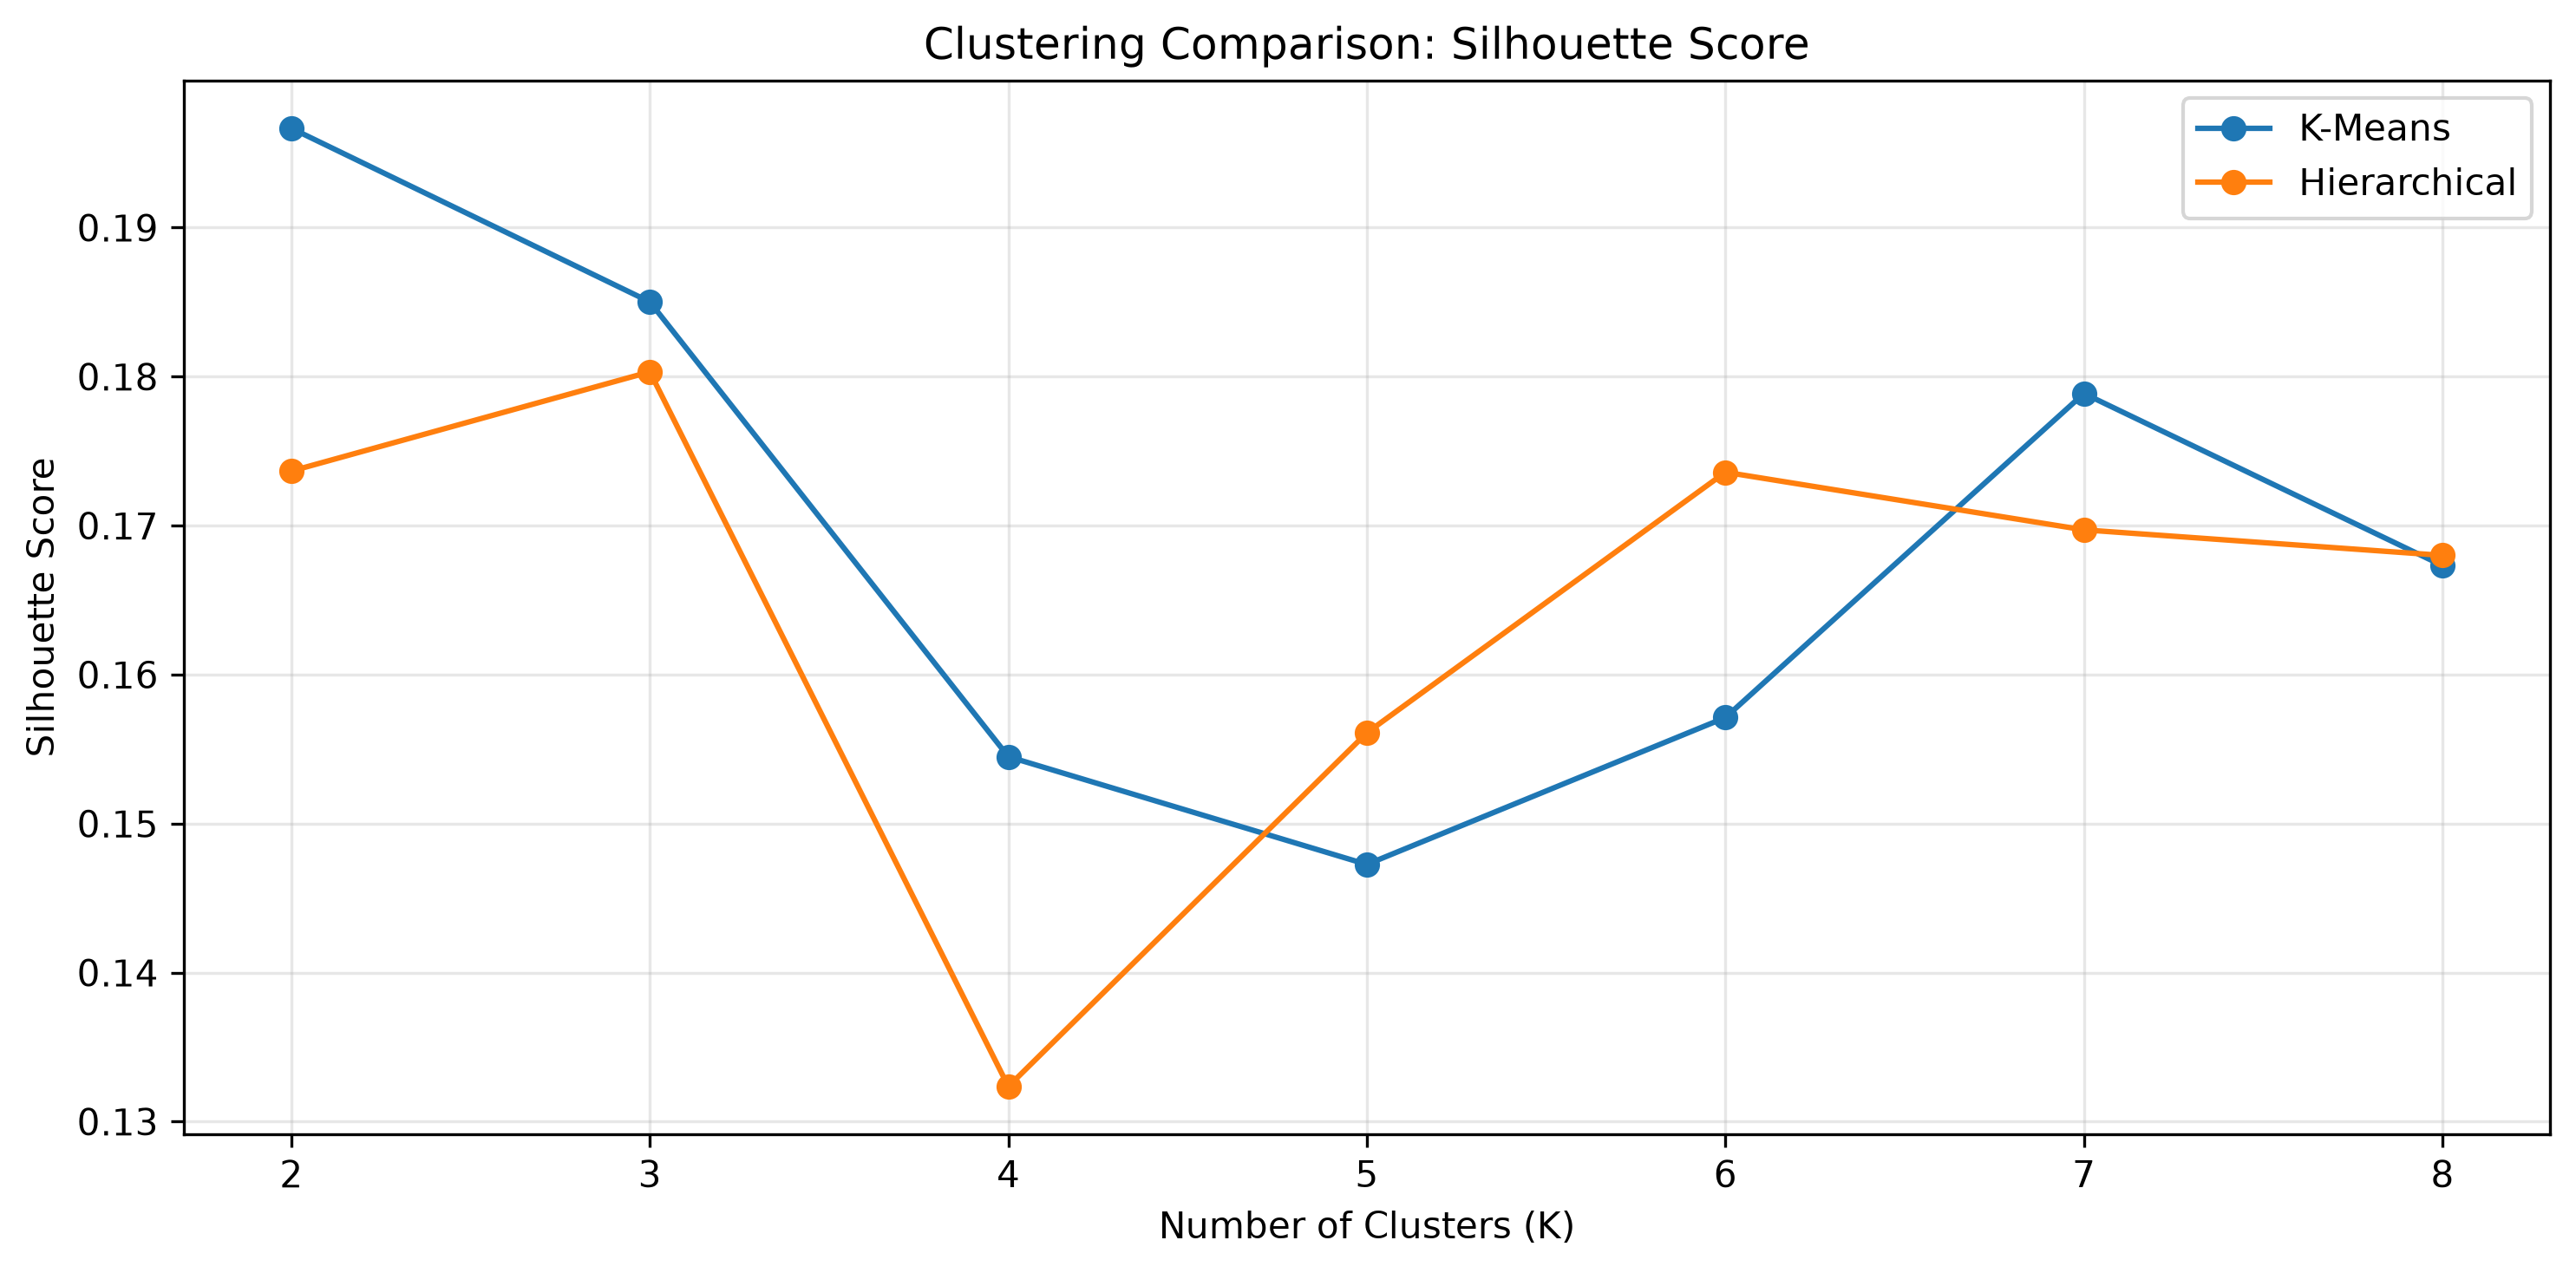
\includegraphics[width=\textwidth]{figures/silhouette_score_comparison.png}
\caption{Silhouette-score comparison for K-Means and hierarchical clustering.}
\label{fig:sil}
\end{figure}

\begin{figure}[H]
\centering
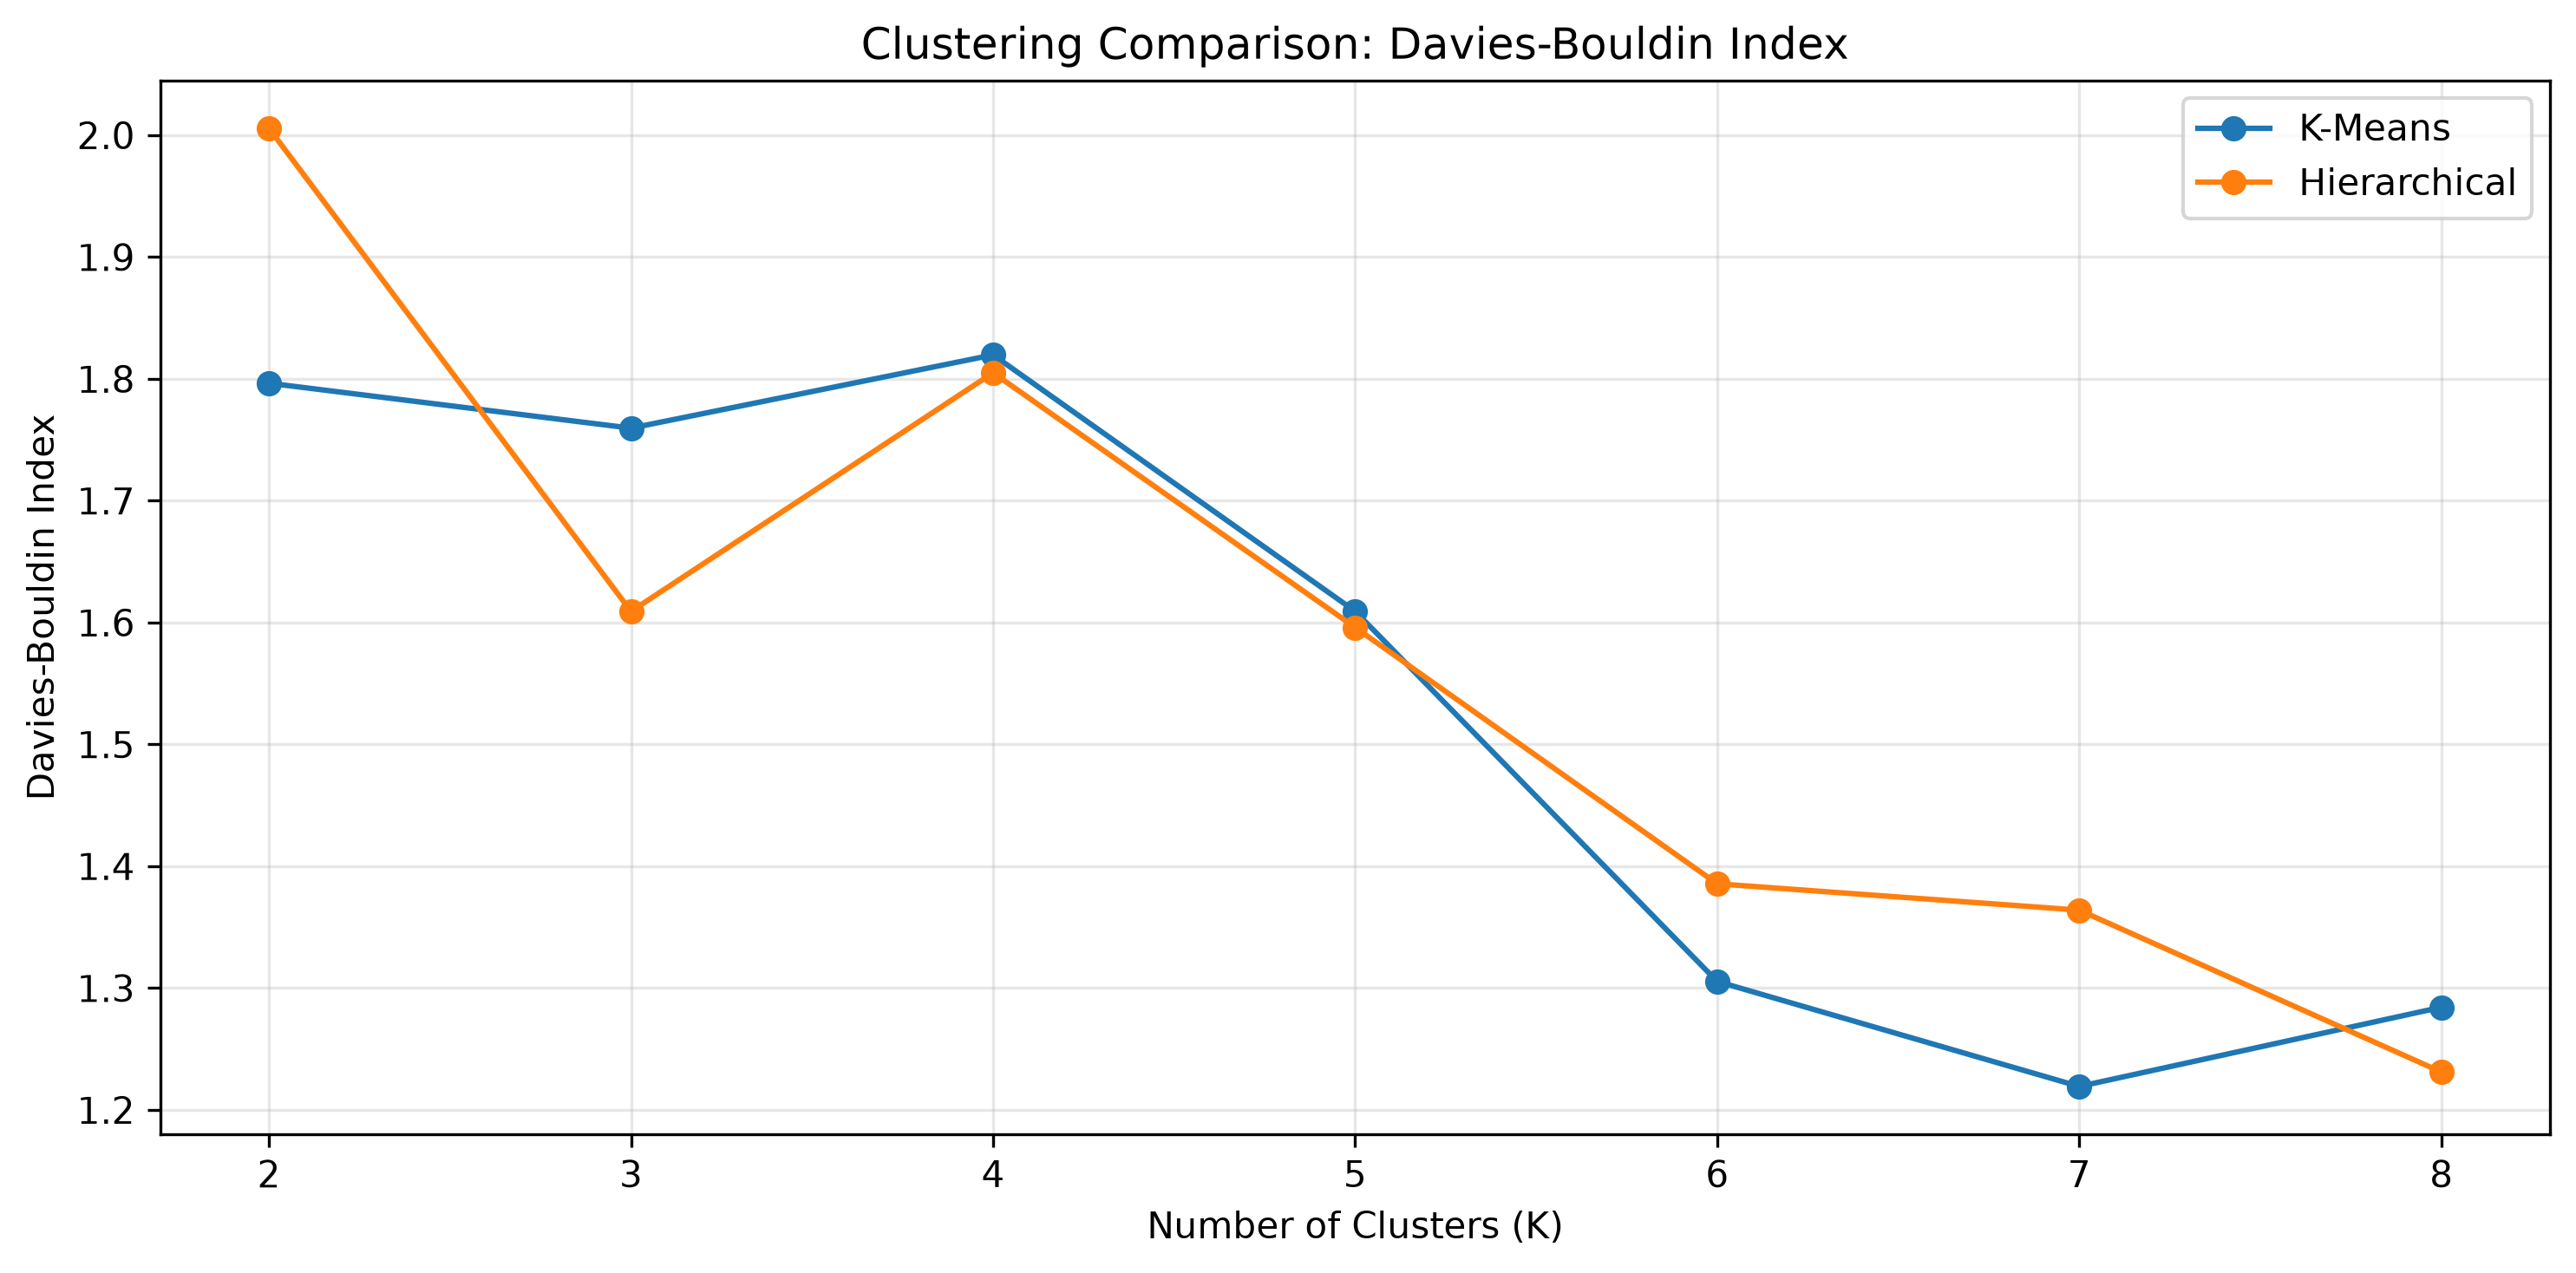
\includegraphics[width=\textwidth]{figures/davies_bouldin_index_comparison.png}
\caption{Davies--Bouldin index comparison. Lower values indicate more compact and separated clusters under this metric.}
\label{fig:db}
\end{figure}

\begin{figure}[H]
\centering
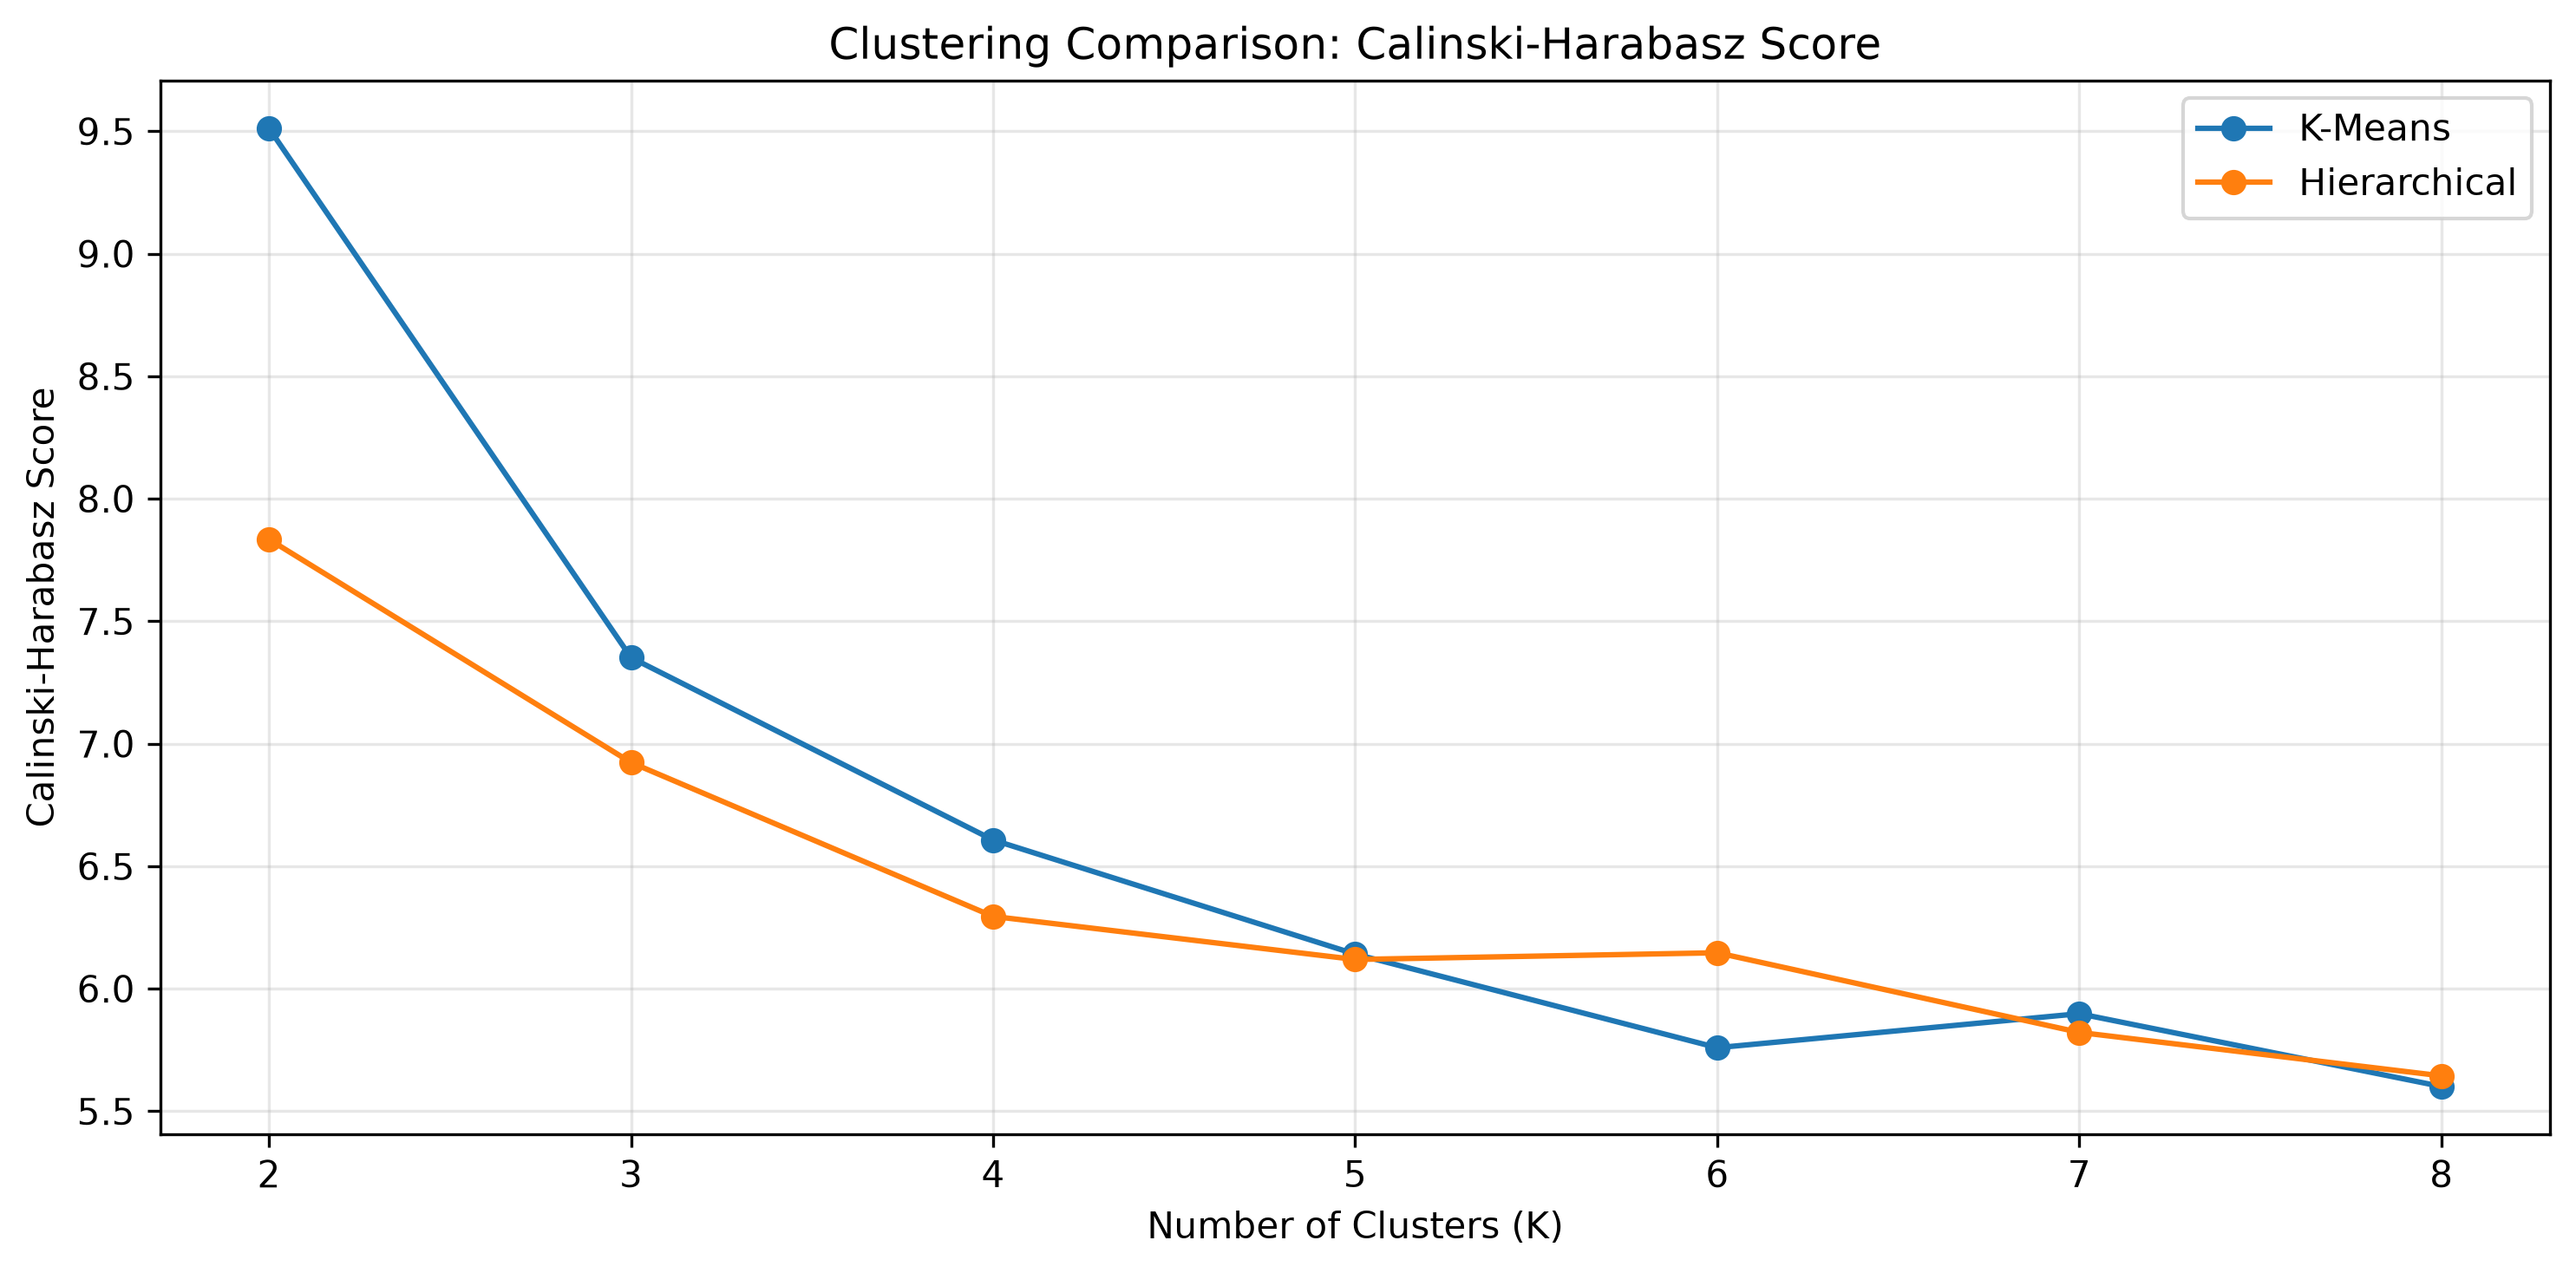
\includegraphics[width=\textwidth]{figures/calinski_harabasz_score_comparison.png}
\caption{Calinski--Harabasz score comparison. Higher values indicate a larger between-cluster to within-cluster dispersion ratio.}
\label{fig:ch}
\end{figure}

\subsection{K-Means stability and baseline comparison}
Table~\ref{tab:stability} summarises the five-seed silhouette results. $K=3$ has the highest mean (0.1970), only slightly above $K=2$ (0.1967). However, $K=2$ has a standard deviation of 0 across the five tested seeds, while the other values of $K$ show non-zero variation. Thus, $K=2$ is the most stable in this limited metric-based test, whereas $K=3$ has the marginally higher average silhouette. The difference is small and should not be interpreted as strong evidence that one value is universally superior.

\begin{table}[H]
\centering
\caption{K-Means silhouette stability across five random seeds.}
\label{tab:stability}
\small
\begin{tabular}{rcc}
\toprule
$K$ & Mean silhouette & Standard deviation\\
\midrule
2 & 0.196670 & 0.000000\\
3 & 0.196973 & 0.006751\\
4 & 0.155157 & 0.012321\\
5 & 0.169360 & 0.012881\\
6 & 0.164156 & 0.013399\\
7 & 0.160292 & 0.016154\\
8 & 0.156232 & 0.008652\\
\bottomrule
\end{tabular}
\end{table}

Table~\ref{tab:baseline} compares the K-Means mean silhouette from the stability experiment with the balanced random-assignment mean. For all tested values of $K$, the K-Means mean is higher than the random baseline mean. This indicates that the observed partitions contain more distance-based structure than the particular balanced random assignments used here. It does not establish statistical significance or rule out alternative null models.

\begin{table}[H]
\centering
\caption{K-Means stability mean compared with the balanced random-assignment baseline.}
\label{tab:baseline}
\small
\begin{tabular}{rccc}
\toprule
$K$ & K-Means mean & Random mean & Random SD\\
\midrule
2 & 0.196670 & 0.000890 & 0.012154\\
3 & 0.196973 & -0.031911 & 0.010777\\
4 & 0.155157 & -0.057709 & 0.010448\\
5 & 0.169360 & -0.077531 & 0.011170\\
6 & 0.164156 & -0.095524 & 0.011988\\
7 & 0.160292 & -0.112500 & 0.013222\\
8 & 0.156232 & -0.125527 & 0.015484\\
\bottomrule
\end{tabular}
\end{table}

\subsection{Cluster membership and profiles}
For an interpretable two-cluster comparison, the saved K-Means and hierarchical assignments at $K=2$ are profiled below. The membership labels are arbitrary identifiers and do not indicate rank.

\textbf{K-Means Cluster 0 (14 regions):} Tripura, West Bengal, Chhattisgarh, Madhya Pradesh, Rajasthan, Uttar Pradesh, Odisha, Arunachal Pradesh, Assam, Meghalaya, Nagaland, Jharkhand, Bihar, and Dadra and Nagar Haveli and Daman and Diu.

\textbf{K-Means Cluster 1 (22 regions):} Kerala, Uttarakhand, Tamil Nadu, Goa, Himachal Pradesh, Punjab, Sikkim, Karnataka, Andhra Pradesh, Gujarat, Telangana, Maharashtra, Haryana, Manipur, Mizoram, Chandigarh, Jammu and Kashmir, Puducherry, Andaman and Nicobar Islands, Delhi, Lakshadweep, and Ladakh.

\textbf{Hierarchical Cluster 0 (15 regions):} Mizoram, Tripura, West Bengal, Chhattisgarh, Madhya Pradesh, Uttar Pradesh, Odisha, Arunachal Pradesh, Assam, Meghalaya, Nagaland, Jharkhand, Bihar, Dadra and Nagar Haveli and Daman and Diu, and Ladakh.

\textbf{Hierarchical Cluster 1 (21 regions):} Kerala, Uttarakhand, Tamil Nadu, Goa, Himachal Pradesh, Punjab, Sikkim, Karnataka, Andhra Pradesh, Gujarat, Telangana, Maharashtra, Haryana, Manipur, Rajasthan, Chandigarh, Jammu and Kashmir, Puducherry, Andaman and Nicobar Islands, Delhi, and Lakshadweep.

The methods produce broadly related but not identical memberships. Rajasthan is assigned to K-Means Cluster 0 but hierarchical Cluster 1; Mizoram and Ladakh are assigned differently between the two methods. This is a reminder that cluster membership depends on the algorithm and its geometry.

Table~\ref{tab:profiles} reports the average original score for every retained goal. The averages are rounded to two decimal places. Goal 14 is not included.

\begin{table}[H]
\centering
\caption{Mean original SDG goal scores by cluster for the two methods.}
\label{tab:profiles}
\scriptsize
\resizebox{\textwidth}{!}{%
\begin{tabular}{llrrrrrrrrrrrrrrr}
\toprule
Method & Cluster & G1 & G2 & G3 & G4 & G5 & G6 & G7 & G8 & G9 & G10 & G11 & G12 & G13 & G15 & G16\\
\midrule
K-Means & 0 & 65.50 & 48.57 & 68.21 & 51.43 & 48.36 & 84.36 & 80.29 & 66.43 & 47.43 & 64.64 & 66.79 & 82.86 & 54.57 & 81.21 & 70.43\\
K-Means & 1 & 74.82 & 69.18 & 77.27 & 68.95 & 56.32 & 91.77 & 97.82 & 74.77 & 61.00 & 70.64 & 80.82 & 68.73 & 63.82 & 73.27 & 77.36\\
Ward & 0 & 65.87 & 49.93 & 67.87 & 51.67 & 50.47 & 87.33 & 81.60 & 68.80 & 47.27 & 63.20 & 64.20 & 78.53 & 56.27 & 79.47 & 72.67\\
Ward & 1 & 75.00 & 69.19 & 77.95 & 69.62 & 55.19 & 90.00 & 97.71 & 73.48 & 61.76 & 71.95 & 83.33 & 71.14 & 63.05 & 74.14 & 76.10\\
\bottomrule
\end{tabular}}
\end{table}

For both methods, Cluster 1 has a higher mean than Cluster 0 on 13 of the 15 retained goals. Cluster 0 has higher means for Goal 12 (Responsible Consumption and Production) and Goal 15 (Life on Land). This is a profile-level description only. It should not be simplified into a claim that one cluster is categorically better, because each group has different goal-specific strengths and weaknesses and the clusters are not official performance labels.

\begin{figure}[H]
\centering
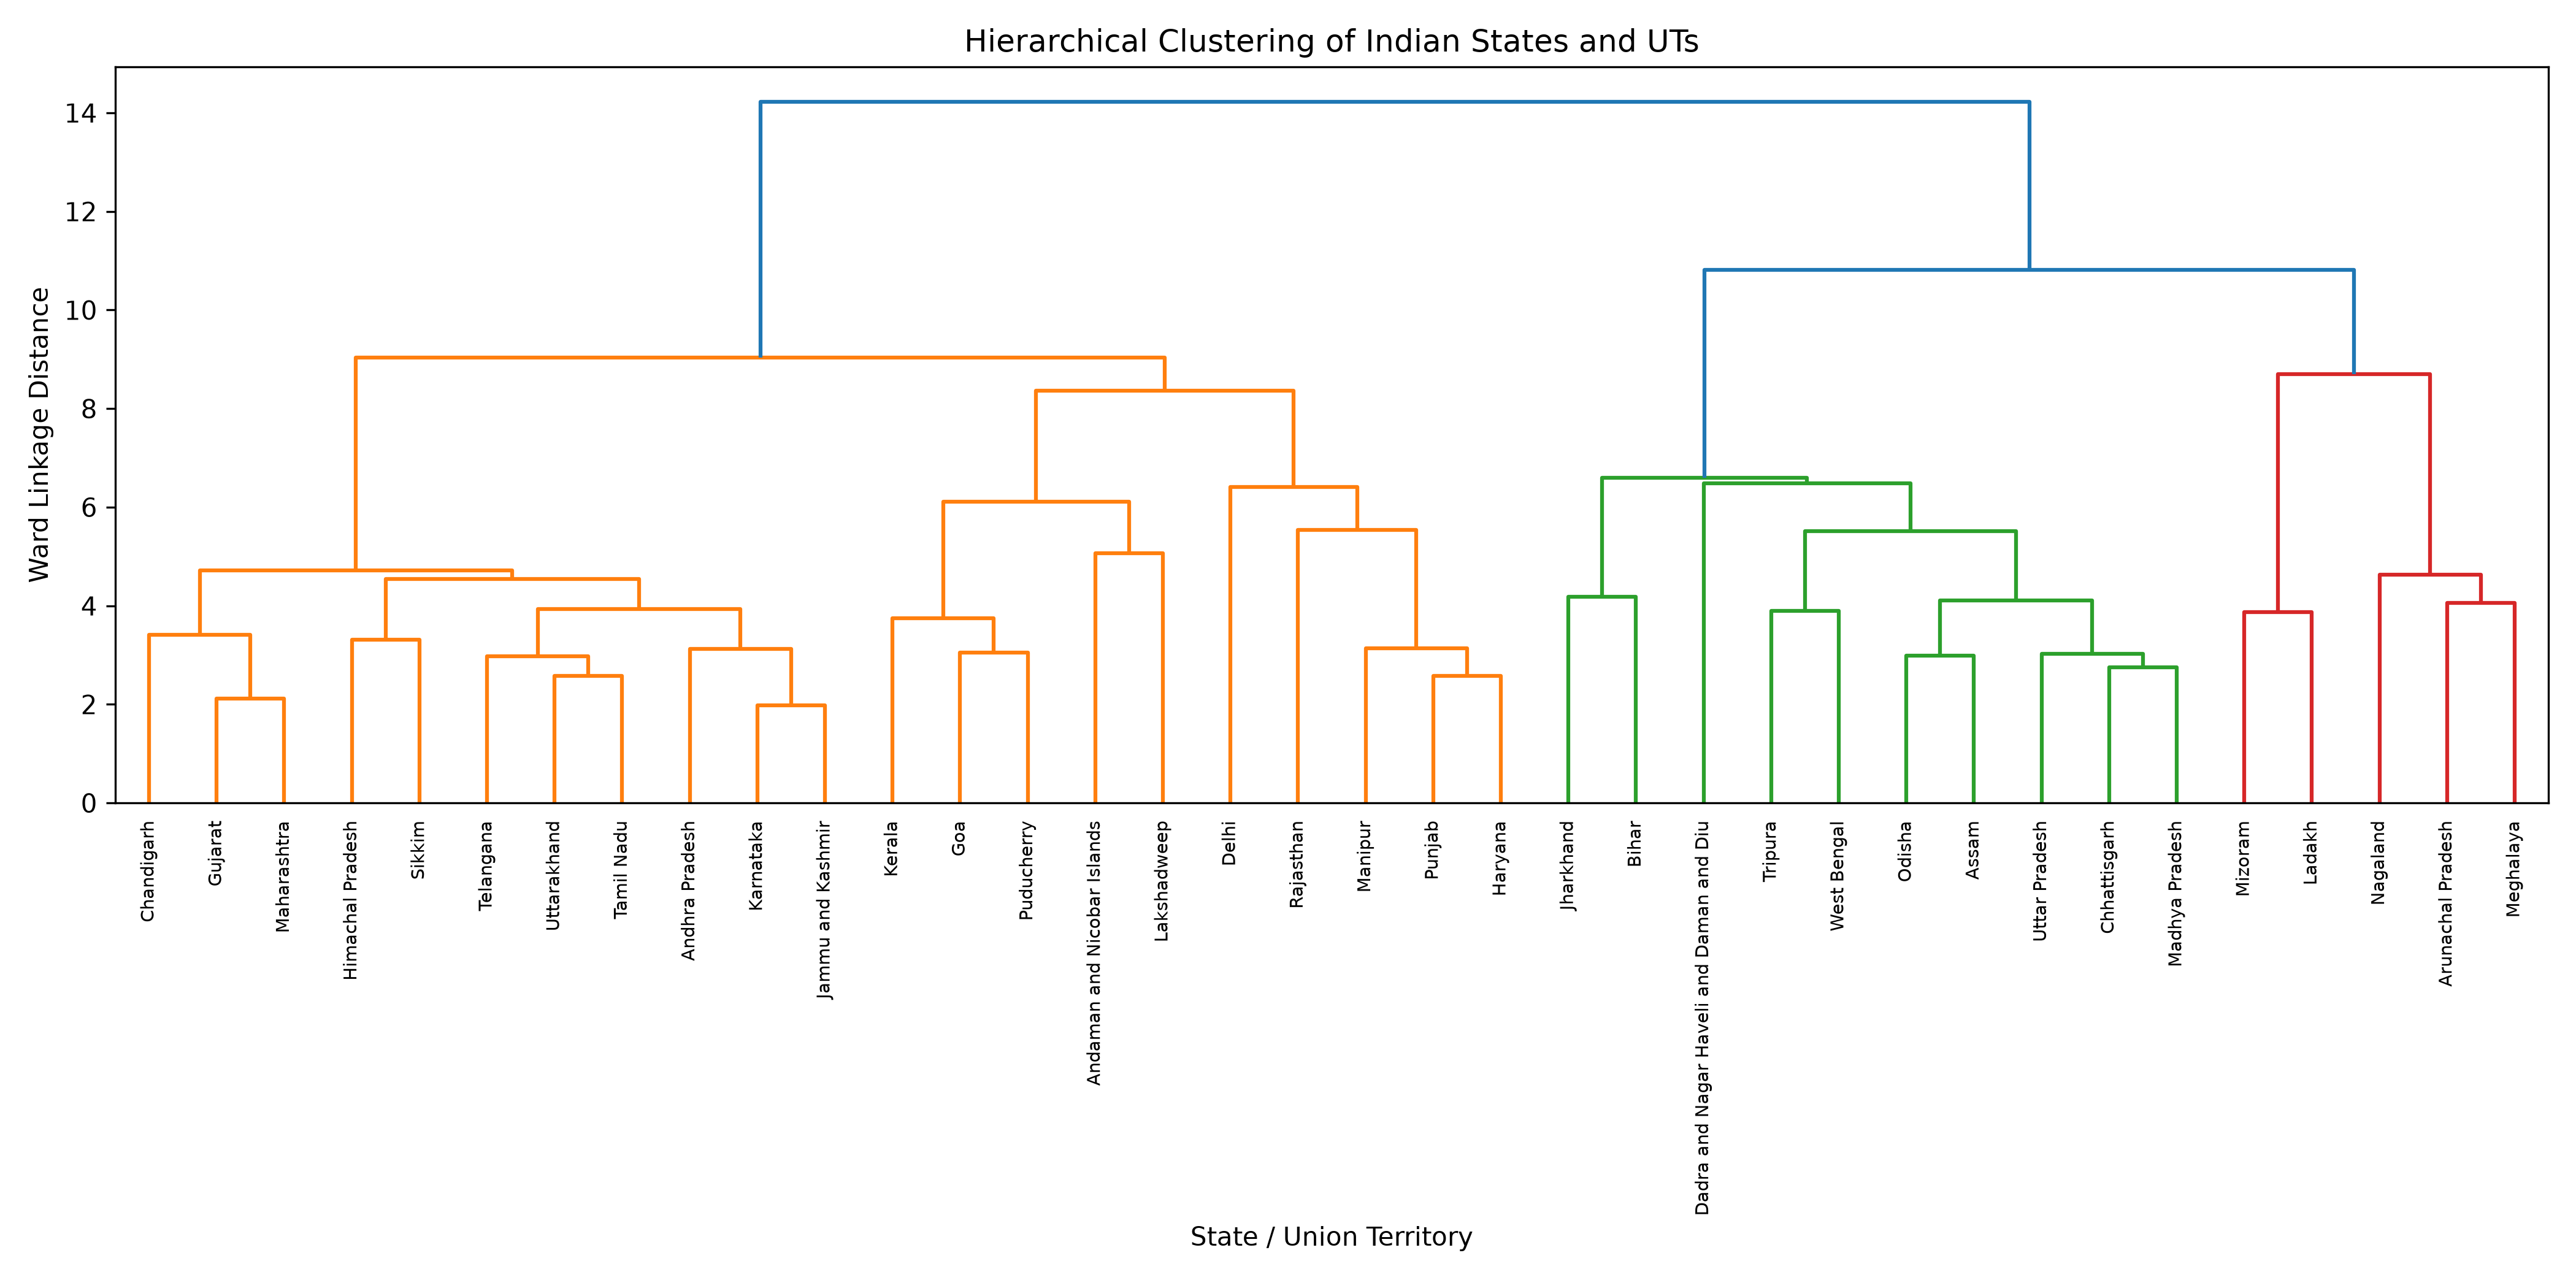
\includegraphics[width=\textwidth]{figures/hierarchical_dendrogram.png}
\caption{Ward-linkage dendrogram for the 36 States and Union Territories using the 15 standardised goal scores.}
\label{fig:dendrogram}
\end{figure}

\subsection{PCA visualisation}
The first two principal components explain 27.27\% and 15.20\% of the total variance, respectively, for a combined 42.47\%. Figure~\ref{fig:pca} plots regions in this two-dimensional projection and colours them by their K-Means $K=2$ membership. Because the first two components retain less than half of the total variance, the plot is a partial projection and should not be treated as proof of clear separation in the full 15-dimensional feature space.

\begin{figure}[H]
\centering
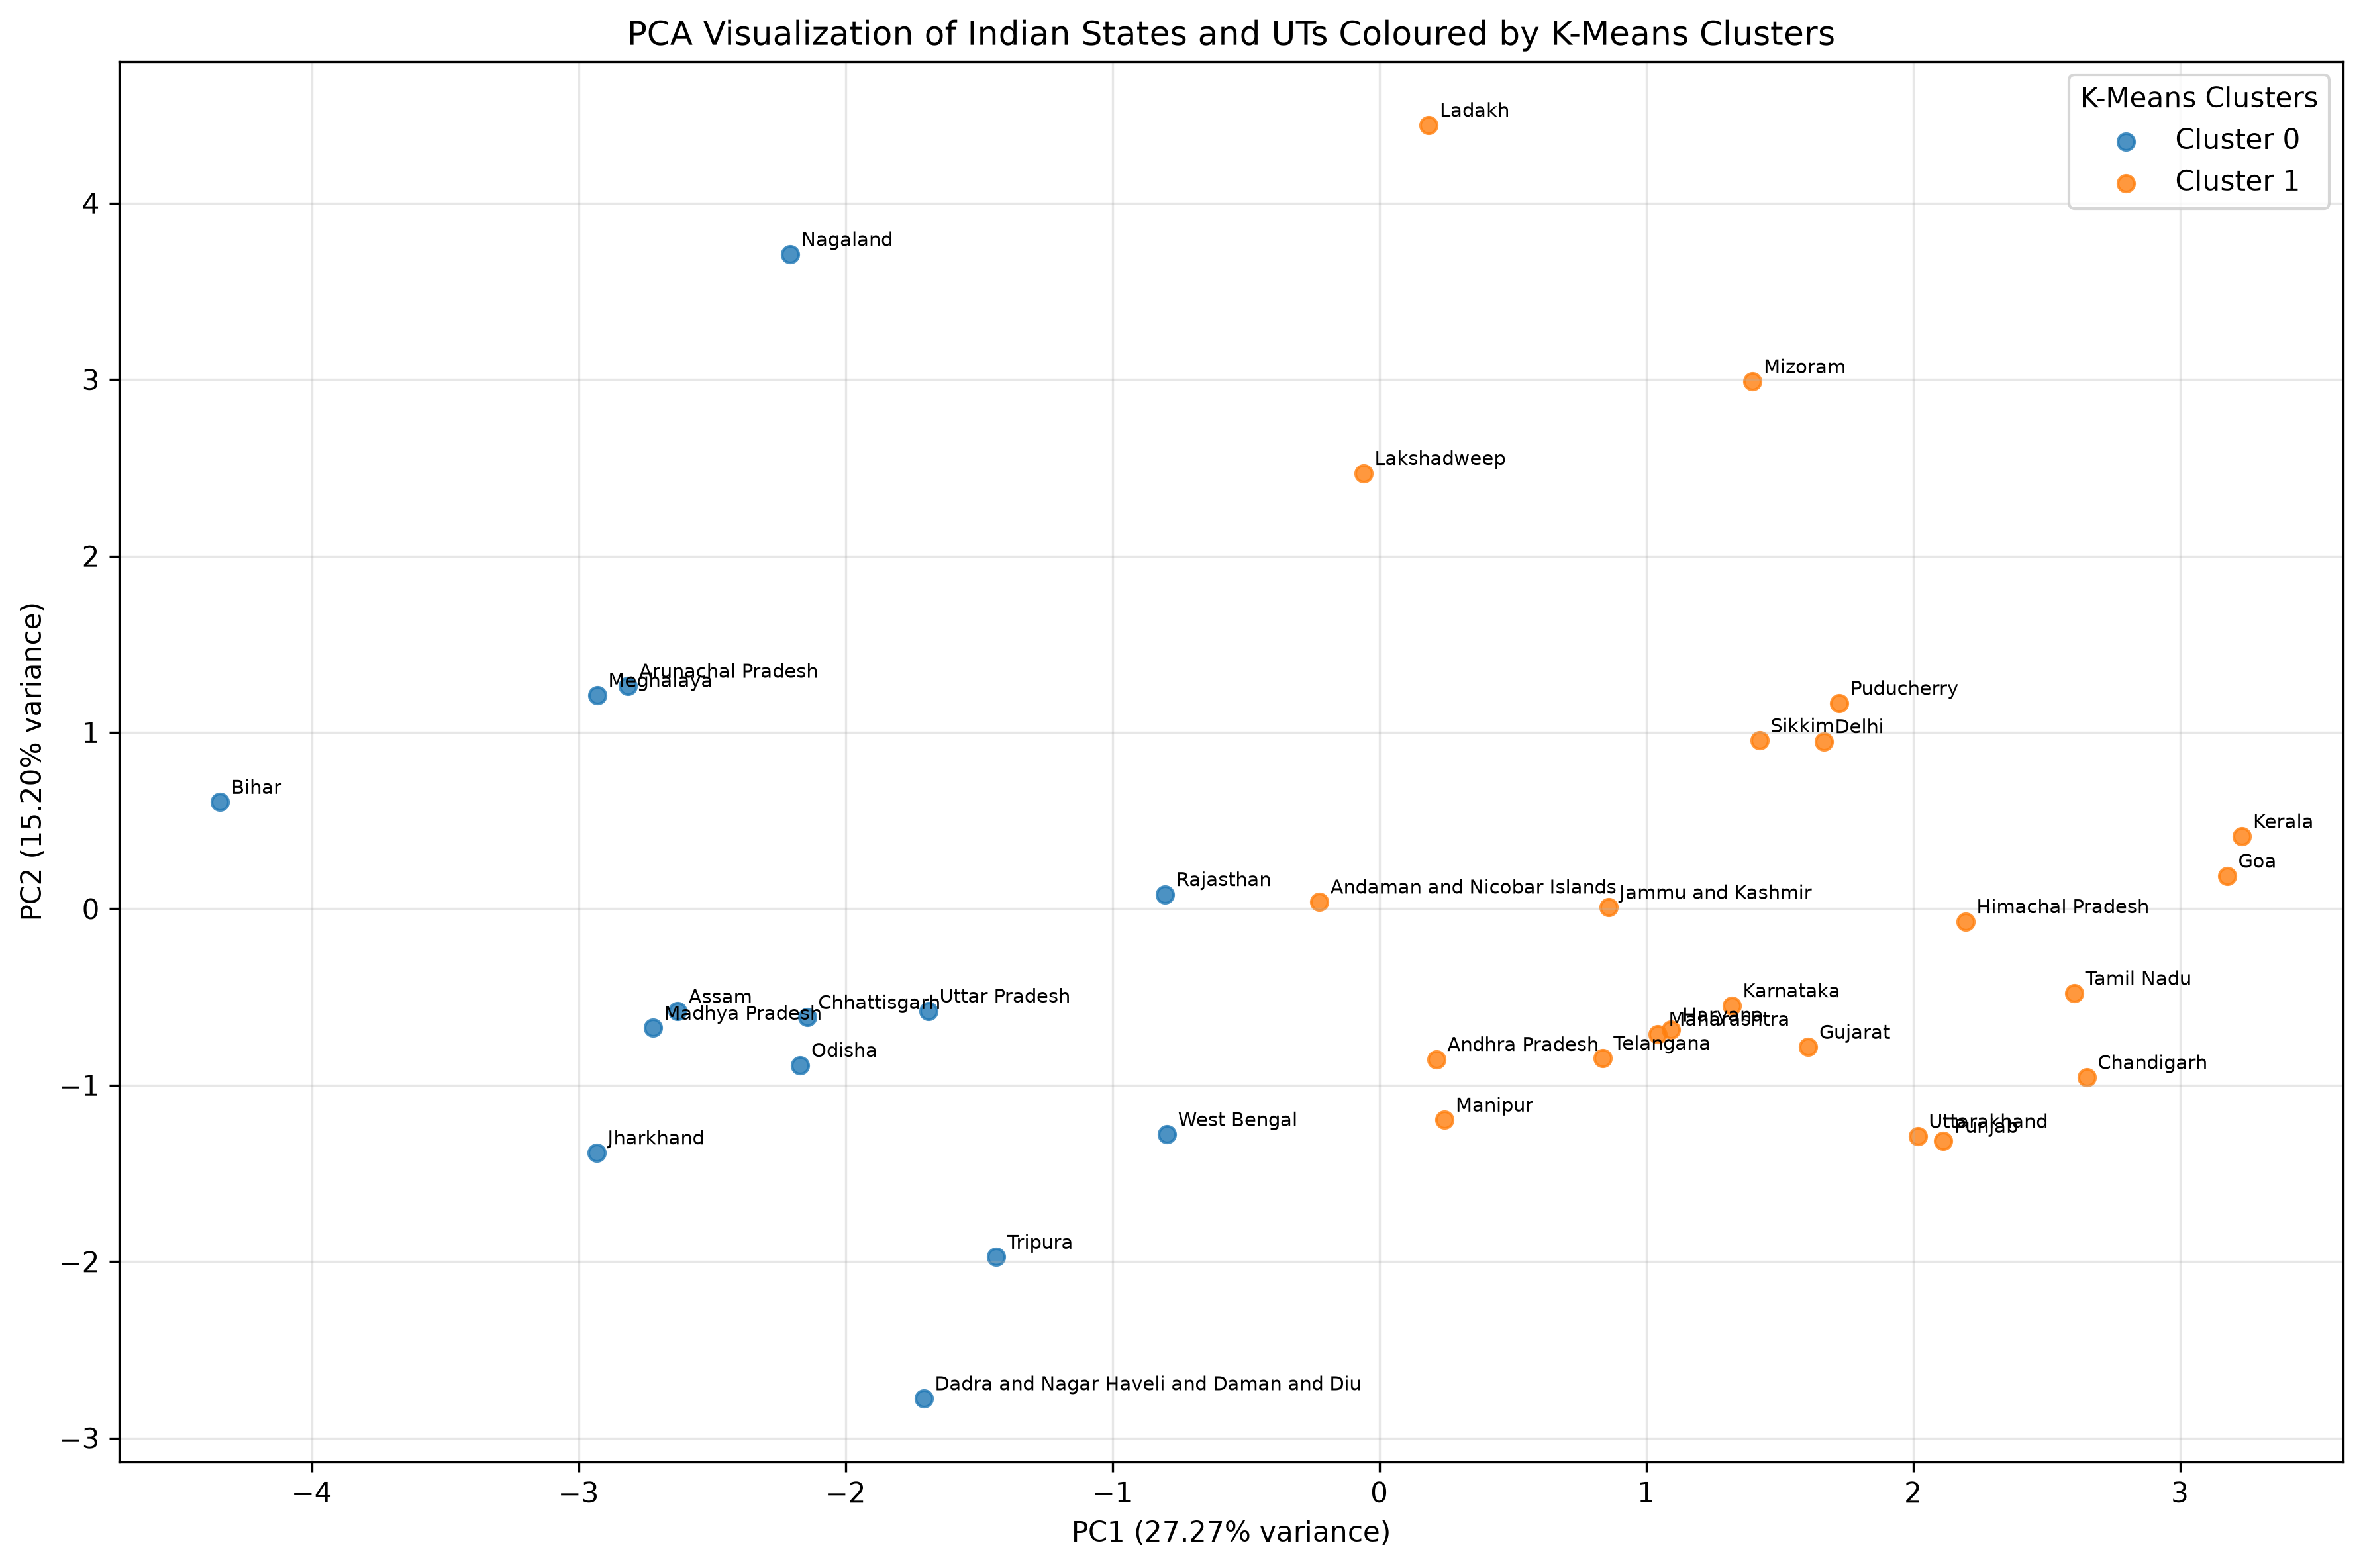
\includegraphics[width=0.95\textwidth]{figures/pca_visualization.png}
\caption{Two-component PCA projection of the 36 regions, coloured by K-Means $K=2$ cluster membership. PC1 explains 27.27\% and PC2 explains 15.20\% of the variance.}
\label{fig:pca}
\end{figure}

\begin{figure}[H]
\centering
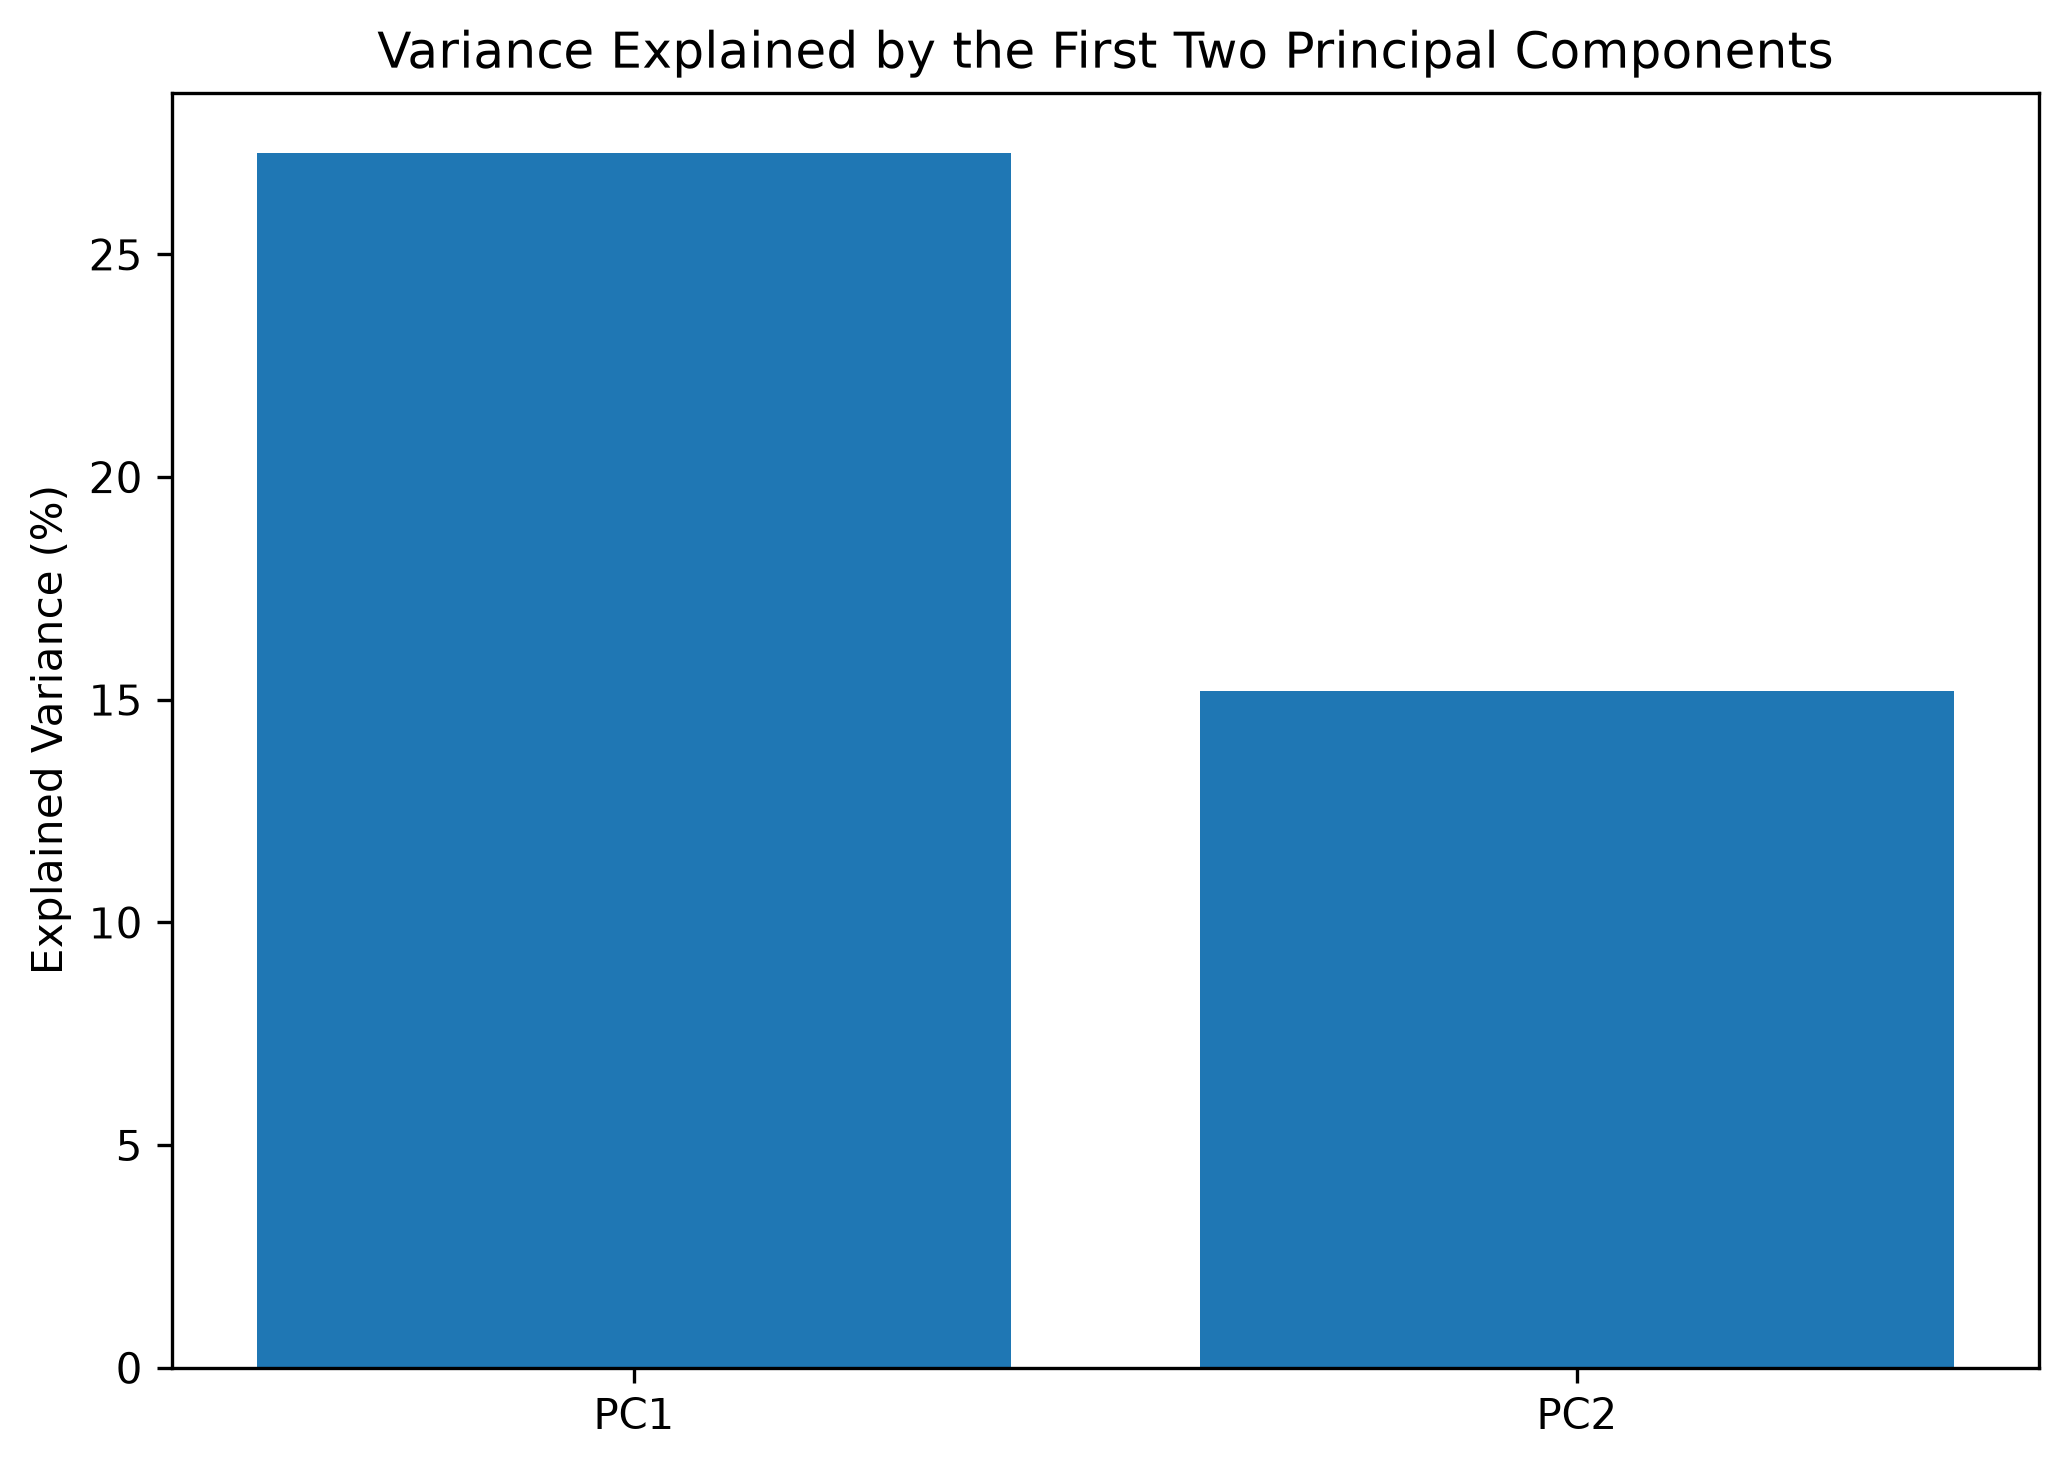
\includegraphics[width=0.65\textwidth]{figures/pca_explained_variance.png}
\caption{Variance explained by the first two principal components.}
\label{fig:pcavar}
\end{figure}

\subsection{PCA-based sensitivity analysis}
The PCA transformation retaining 90\% of variance reduces the feature representation from 15 standardised goal scores to nine principal components and retains 90.06\% of the variance. Table~\ref{tab:pcasens} compares K-Means on the original and reduced representations. For $K=2$, ARI is 1.0000, meaning the two methods produce the same partition up to cluster-label permutation. For other values of $K$, ARI varies, indicating that dimensionality reduction can alter assignments.

\begin{table}[H]
\centering
\caption{K-Means comparison between original standardised features and PCA-reduced features.}
\label{tab:pcasens}
\scriptsize
\begin{tabular}{rccccccc}
\toprule
$K$ & Orig. Sil. & PCA Sil. & Orig. DB & PCA DB & Orig. CH & PCA CH & ARI\\
\midrule
2 & 0.1967 & 0.2238 & 1.7964 & 1.6517 & 9.5119 & 10.8341 & 1.0000\\
3 & 0.1850 & 0.2302 & 1.7595 & 1.4404 & 7.3515 & 8.9989 & 0.8927\\
4 & 0.1545 & 0.2004 & 1.8197 & 1.4753 & 6.6071 & 8.0161 & 0.8641\\
5 & 0.1473 & 0.1894 & 1.6092 & 1.4984 & 6.1412 & 7.4308 & 0.6714\\
6 & 0.1571 & 0.1788 & 1.3054 & 1.3423 & 5.7591 & 7.0301 & 0.6726\\
7 & 0.1789 & 0.2264 & 1.2192 & 1.0615 & 5.8979 & 7.2826 & 0.9349\\
8 & 0.1673 & 0.1840 & 1.2842 & 1.2250 & 5.6008 & 6.8247 & 0.7375\\
\bottomrule
\end{tabular}
\end{table}

The PCA-reduced representation produces higher silhouette and Calinski--Harabasz scores for each tested $K$ in this experiment. Its Davies--Bouldin index is lower for all tested values except $K=6$. These results suggest that PCA can provide a useful alternative representation for this dataset. However, PCA components are linear combinations of the original goals and are less directly interpretable; the comparison does not establish that PCA is universally preferable or that it assigns policy weights to individual goals.

\subsection{Correlation analysis}
Pearson correlations are calculated among the 15 retained goal scores. The strongest positive correlation in the observed matrix is between Goal 4 and Goal 9 ($r=0.67$), while the strongest negative correlation is between Goal 5 and Goal 12 ($r=-0.55$). Other notable positive correlations include Goal 2 with Goal 4 ($r=0.53$), Goal 4 with Goal 11 ($r=0.52$), and Goal 3 with Goal 9 ($r=0.51$). These are associations within this 36-region dataset and do not establish causal relationships.

\begin{figure}[H]
\centering
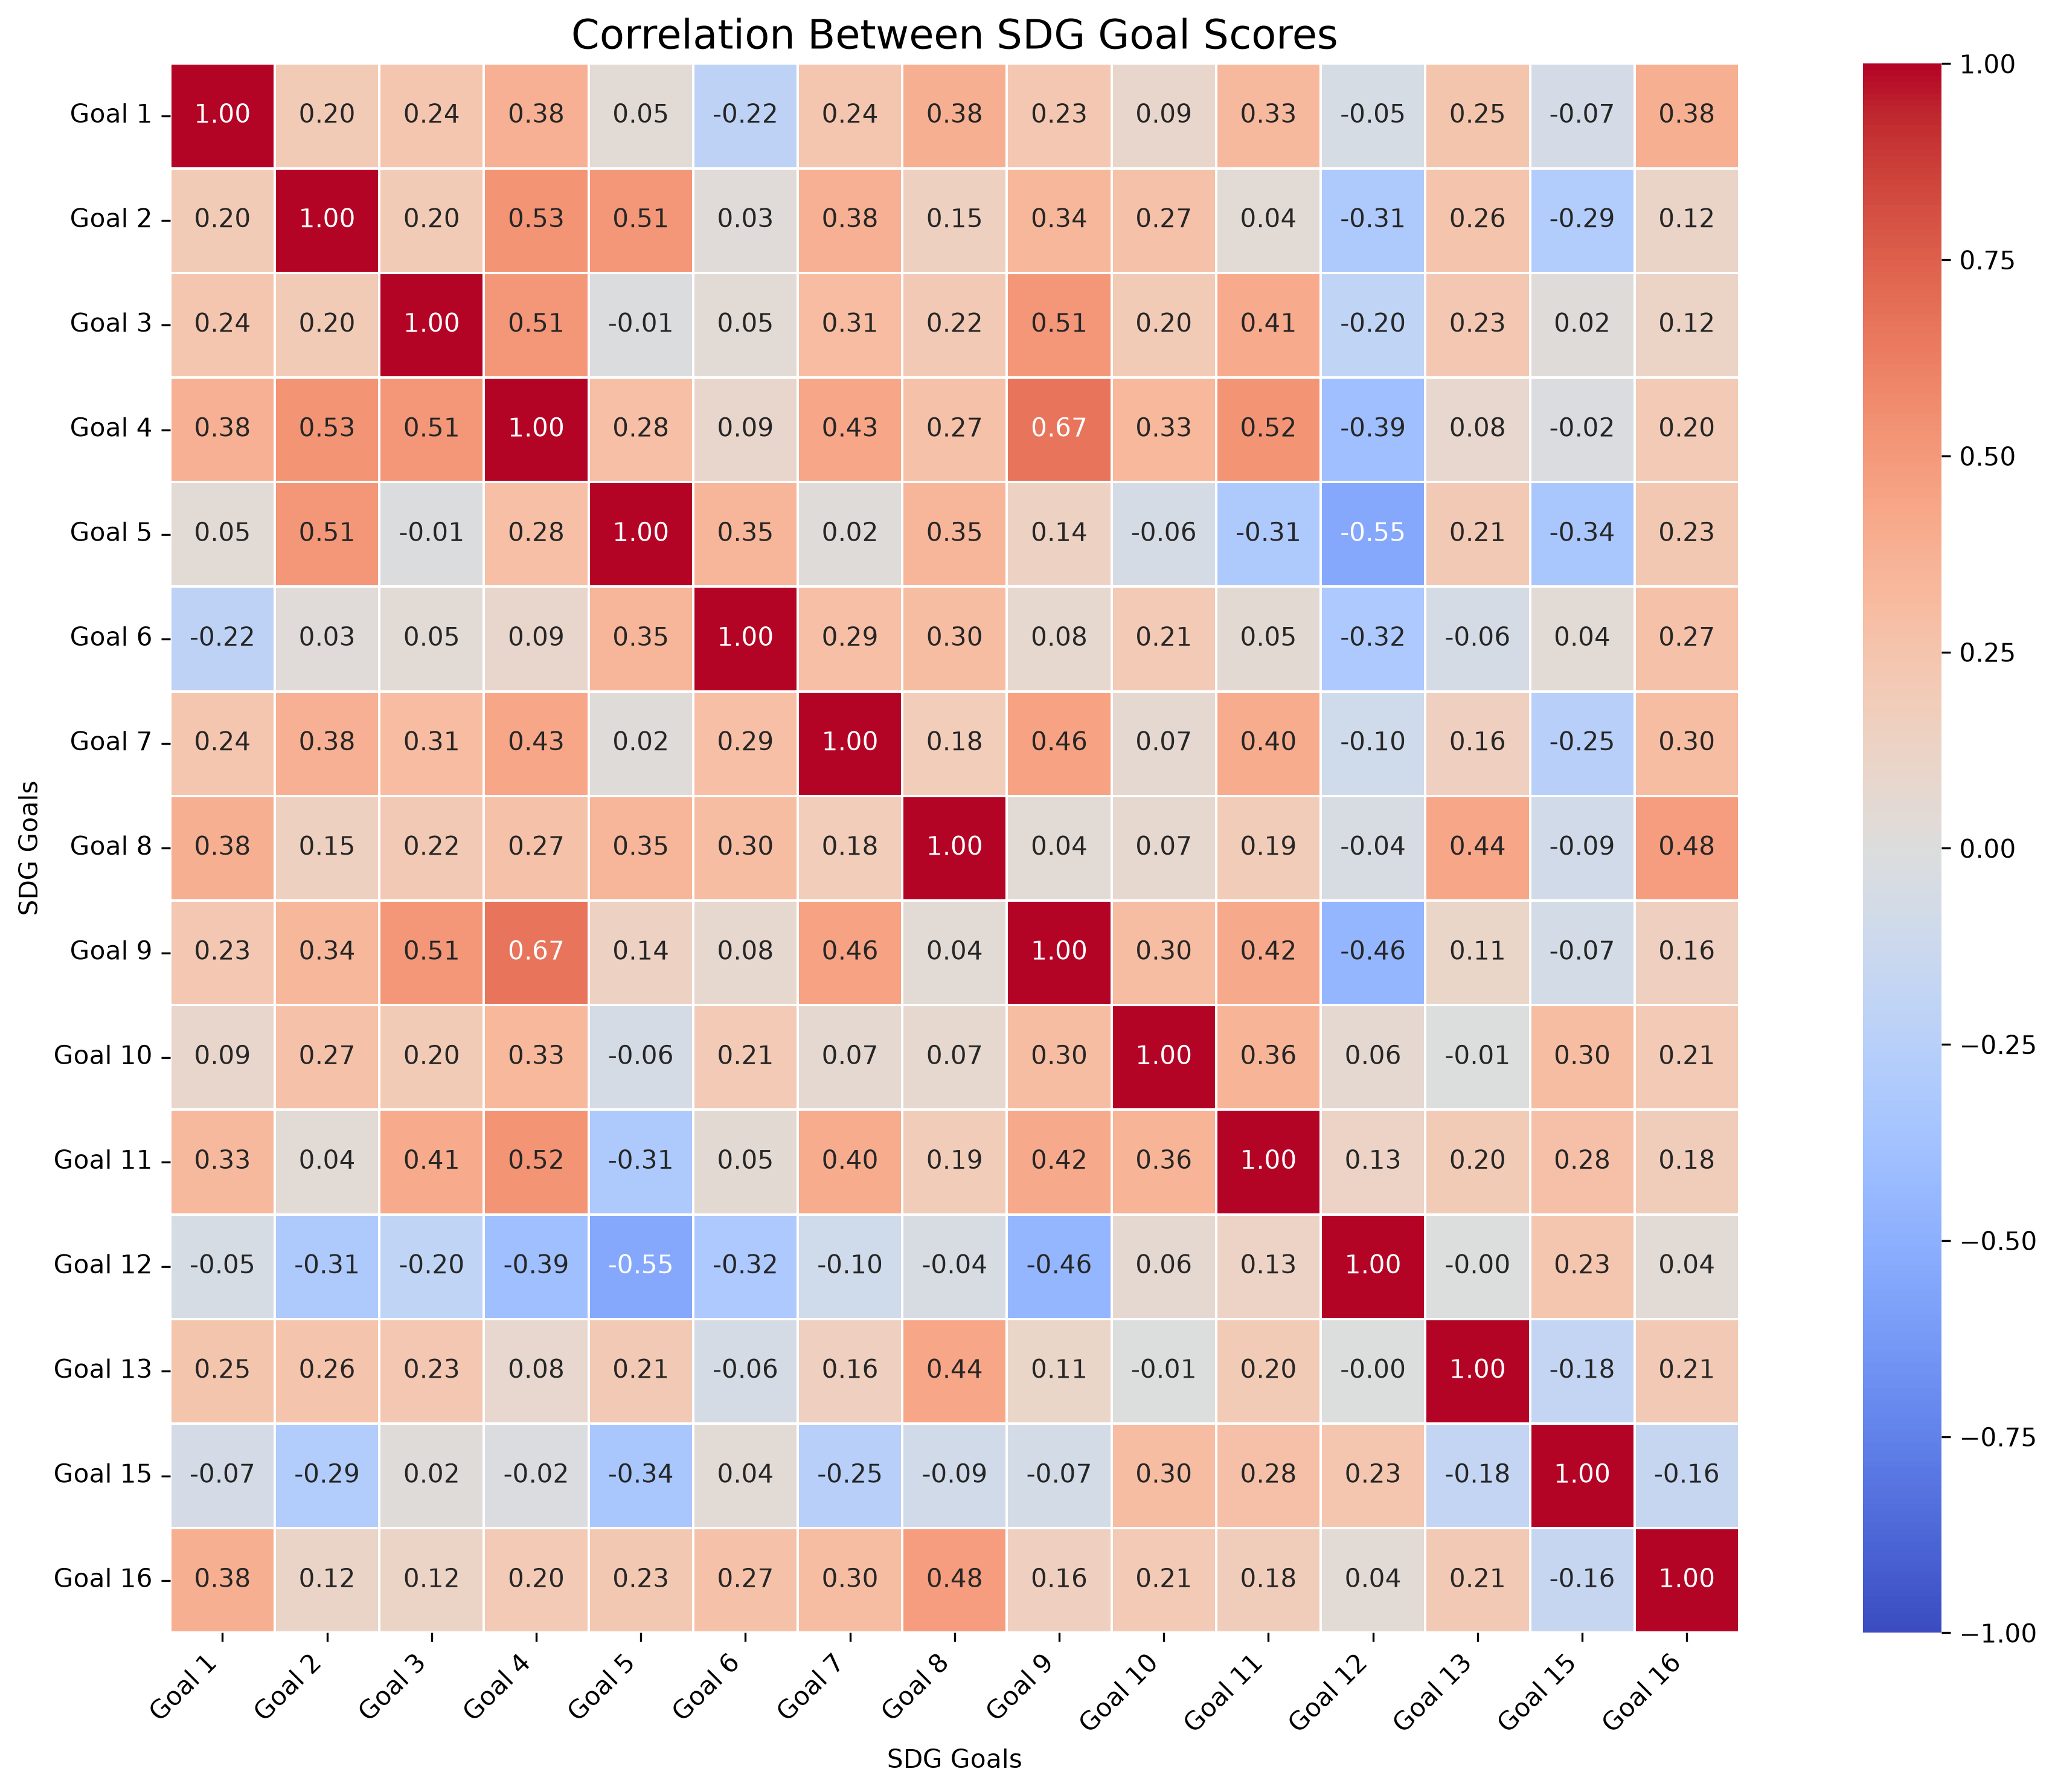
\includegraphics[width=0.92\textwidth]{figures/sdg_correlation_heatmap.png}
\caption{Pearson correlation heatmap for the 15 retained SDG goal scores.}
\label{fig:corr}
\end{figure}

\subsection{Exploratory outlier screening}
Isolation Forest flags four regions as potential outliers under the selected contamination setting of 0.10: Nagaland, Bihar, Delhi, and Dadra and Nagar Haveli and Daman and Diu. The result identifies observations with unusual multivariate combinations of goal scores relative to the dataset. It does not mean that these regions are erroneous, deficient or intrinsically anomalous. The flagged cases should be checked against source data, indicator definitions and regional context before any substantive interpretation.

\section{Discussion}
The results indicate modest cluster separation: the observed silhouette scores are positive but relatively low. K-Means at $K=2$ provides the strongest single-seed silhouette result and highest Calinski--Harabasz score among the tested K values, while the Davies--Bouldin index favours a larger K. The five-seed summary shows that $K=3$ has a marginally higher mean silhouette, whereas $K=2$ has no observed silhouette variation across the tested seeds. These results support presenting $K=2$ as a stable and interpretable comparison rather than asserting that it is the unique optimal solution.

The two clustering methods share broad profile patterns but differ for a small number of regions. The profile averages show that clusters have different goal-specific strengths, which is precisely why a single composite score or cluster label should not be used as a complete account of development. The balanced random baseline provides a useful reference: the observed K-Means silhouette means exceed the baseline means at every tested K. Nevertheless, the baseline is simple and does not replace permutation testing, alternative null models or external validation.

The PCA sensitivity analysis shows that reducing the feature space to nine components can improve internal metrics for this dataset, while preserving the $K=2$ partition exactly (ARI=1.0000). The two-dimensional PCA plot, however, retains only 42.47\% of variance. It is therefore useful for visual inspection but cannot fully represent all distances and relationships in the original feature space.

\section{Limitations and Future Work}
This study has several limitations:
\begin{enumerate}[leftmargin=1.5em]
  \item \textbf{Missing Goal 14 data:} 27 of 36 values are missing in the analysed CSV, so the goal is excluded. Future work could examine a validated coastal-state-only analysis or obtain a suitable comparable dataset.
  \item \textbf{Small sample:} 36 regions provide a limited number of observations for high-dimensional clustering with 15 features.
  \item \textbf{Single reporting period:} The analysis is cross-sectional and does not model changes over time.
  \item \textbf{Metric disagreement and modest separation:} Internal validation metrics do not identify one universally best K, and silhouette values indicate limited separation.
  \item \textbf{Baseline scope:} The balanced random baseline is a simple reference and not a comprehensive statistical null model.
  \item \textbf{Stability scope:} Five random seeds assess silhouette-score variation but do not fully quantify membership stability using measures such as pairwise adjusted Rand indices.
  \item \textbf{Outlier parameter:} Isolation Forest's contamination value of 0.10 is an analyst-selected setting; outlier flags require independent validation.
  \item \textbf{Feature influence:} Standardisation addresses scale differences but does not remove correlation or guarantee equal effective influence of each goal.
  \item \textbf{Interpretability:} PCA components combine multiple goals and are less directly interpretable than the original goal scores.
\end{enumerate}

Future work could incorporate multiple Index editions, compare additional clustering algorithms, evaluate membership stability with adjusted Rand or consensus methods, test alternative baseline models, and conduct sensitivity analysis using domain-informed feature weights. A larger or more granular district-level dataset could provide more detailed insights, provided that data definitions and coverage are comparable.

\section{Ethical Considerations}
The cluster labels are analytical groupings generated from the selected data and modelling choices. They are not official categories, rankings, or judgements about the quality of governance or the people living in a region. A region's membership can change when the feature set, scaling, period, algorithm or number of clusters changes. Potential outlier labels are similarly exploratory. Any policy use should include local context, data-quality review, stakeholder consultation and examination of individual SDG indicators. The analysis should support investigation and discussion, not be used alone to determine funding, eligibility or public evaluation.

\section{Conclusion}
This study used K-Means and Ward-linkage hierarchical clustering to explore similarities among 36 Indian States and Union Territories using 15 complete SDG India Index goal scores. K-Means achieved a single-run maximum silhouette of 0.1967 at $K=2$, while the five-seed mean was marginally highest at $K=3$; $K=2$ showed zero silhouette standard deviation across the tested seeds. The balanced random baseline had lower mean silhouette scores for all tested K values. Cluster profiles identified goal-specific differences, and the two algorithms produced similar but non-identical memberships. PCA reduced the feature space to nine components while retaining 90.06\% variance; the two-dimensional visualisation explained 42.47\%. Four regions were flagged for exploratory outlier review. Overall, clustering offers a complementary descriptive view of subnational SDG profiles, but the modest separation, missing Goal 14 data and sensitivity to modelling choices require cautious interpretation.

\section*{Data and Code Availability}
The analysis scripts and project outputs are maintained in the author's project repository:
\url{https://github.com/Vidhimaheshwari013/ML-Project}.
The dataset used in the project is based on the SDG India Index 2023--24 publication and associated state/UT score data from NITI Aayog. No credentials, private information or API keys are required to reproduce the analysis.

\section*{Declaration}
This article reports an academic analysis conducted as part of a Machine Learning project. The interpretations are the author's and do not represent official classifications issued by NITI Aayog or the Government of India.

\bibliographystyle{plainnat}
\bibliography{references}

\end{document}
